\documentclass[12pt]{report} % or report, article, etc.

%%%%%%%%%%%%%%%%%%%%%%%%%%%%%%%%%%%%%%%%%%%
% Math Packages
\usepackage{amsfonts}
\usepackage{amsmath}                     
\usepackage{amssymb}                      
\usepackage{amsthm}
\usepackage{mathtools}
\usepackage{centernot}
%%%%%%%%%%%%%%%%%%%%%%%%%%%%%%%%%%%%%%%%%%%s

%%%%%%%%%%%%%%%%%%%%%%%%%%%%%%%%%%%%%%%%%%%
% Page Layout and Formatting Packages
\usepackage[a4paper, 
            margin=0.75in, 
            headheight=15pt, 
            headsep=0.2in, 
            footskip=1.5cm]{geometry} 
\usepackage{fancyhdr}
\usepackage{hyperref}
\usepackage{bookmark}
\usepackage{graphicx}
\usepackage{enumitem}
\usepackage{tikz}
\usepackage{tcolorbox}
\usepackage{lastpage} % Added for page reference in footer
\usepackage{tocloft} % For customizing ToC spacing
\usepackage{algorithm}
\usepackage{algpseudocode}
\setlength{\cftbeforesecskip}{8pt} % Adjust spacing between section entries
%%%%%%%%%%%%%%%%%%%%%%%%%%%%%%%%%%%%%%%%%%%

%%%%%%%%%%%%%%%%%%%%%%%%%%%%%%%%%%%%%%%%%%%
% Header and Footer Configuration
\pagestyle{fancy} 
\fancyhead[L]{\textbf{CMOR 504 - Graph Theory}}
\fancyhead[C]{}
\fancyhead[R]{}

\renewcommand{\headrulewidth}{0.5pt} % headline (line in header)
\renewcommand{\footrulewidth}{0.5pt} % footline (line in footer) 

\fancyfoot[L]{\textbf{Dr. Randy L. Dalvia}} 
\fancyfoot[C]{} 
\fancyfoot[R]{\textbf{Page \thepage \text{} of \pageref*{LastPage}}}

\title{
    \textbf{\Huge{CMOR 504 \\ Project Report}} \\ [0.5em] 
    \Large {\color{gray} 
        \textbf{Project Report} \\
        \emph{Non-Isomorphic Local Complement Branch and Bound Scheme and its Applications to Graph Theory Fundamentals}
    } \\[1em]
    \large{\textit{Version 1.0.0}}
}
\author{\LARGE{Axel Sanchez Moreno}}
\date{Last Updated: \\ \vspace{0.25em} \large{\textit{\today}}}
%%%%%%%%%%%%%%%%%%%%%%%%%%%%%%%%%%%%%%%%%%%

%%%%%%%%%%%%%%%%%%%%%%%%%%%%%%%%%%%%%%%%%%%
% Font Configuration
\renewcommand{\familydefault}{\sfdefault}

\usepackage{titlesec}
\titleformat*{\section}{\huge\bfseries}
%%%%%%%%%%%%%%%%%%%%%%%%%%%%%%%%%%%%%%%%%%%

%%%%%%%%%%%%%%%%%%%%%%%%%%%%%%%%%%%%%%%%%%
% Format Packages
\setlength{\parindent}{0pt}
%%%%%%%%%%%%%%%%%%%%%%%%%%%%%%%%%%%%%%%%%%%

%%%%%%%%%%%%%%%%%%%%%%%%%%%%%%%%%%%%%%%%%%%
% Color labeling
% Remark/Note:  colback=yellow!10!white,colframe=orange!75!black,title = \Large \textbf{Remark}
% Definition:   colback=teal!10!white,colframe=blue!75!black,title = \Large \textbf{Definition}
% Theorem:      colback=yellow!10!white, colframe=red!75!black, title=\Large \textbf{Theorem}
%%%%%%%%%%%%%%%%%%%%%%%%%%%%%%%%%%%%%%%%%%%

%%%%%%%%%%%%%%%%%%%%%%%%%%%%%%%%%%%%%%%%%%%
% Custom Commands
\newcommand{\argmin}{\operatorname{argmin}}
\newcommand{\feasible}{\operatorname{feasible}}
%%%%%%%%%%%%%%%%%%%%%%%%%%%%%%%%%%%%%%%%%%%

\begin{document}

\maketitle

\newpage

\thispagestyle{empty} % Skip header and footer on this page

\vspace*{\fill}
\begin{center}
    \Large \textbf{This Page is Intentionally Left Blank}
\end{center}
\vspace*{\fill}

\clearpage
\pagenumbering{arabic}
\setcounter{page}{1}

%%%%%%%%%%%%%%%%%%%%%%%%%%%%%%%%%%%%%%%%%%%%%%%%%%%%%%%%%%%%
\newpage
%%%%%%%%%%%%%%%%%%%%%%%%%%%%%%%%%%%%%%%%%%%%%%%%%%%%%%%%%%%%

\begin{tcolorbox}[colback=orange!10!white, colframe=orange!75!black, title=\center \Large \textbf{Abstract}]
    Recent work in quantum computing focuses on understanding qubits in the lense of graph theory. One such operation includes the local complement. Despite its simple definiton, it can be become a redundant task if the graph is presumed to be dense and have local complements 
    that are isomorphic to previous graphs. We're focused on constructing a recursive algorithm that finds all non-isomorphic graphs from the initial-state graph. Given the final listing of all the non-isomorphic graphs, we'll proceed to quantify the various properties of each 
    graph including maximum stable set, maximum cliques, matchings, and perfect matchings. 
\end{tcolorbox}

\subsection*{Introduction}

% Graph states in \cite{Vesperini_2024} act as a connection between qubits and both computing and communication. Recent work from \cite{Adcock_2020} bridges the connection via local complements on graph states. Despite the process of computing the local complement of a graph 
% to be simple, the challenge can become when a larger number of qubits that have dense connections between eachother and, as a result, to collect results on such unique local complemetary graphs. Hence, we propose a recursive algorithm that finds all non-isomorphic graphs to the original graph state. 

Graph states in \cite{Vesperini_2024} connect qubits and both their computation and communication. One such focus comes from \cite{Adcock_2020} on the use of local complements as a transformation on the original stated graph. Despite the local complement operation being straightforward,
finding all possible combinations of such local complements can be challenging when the node count is large or the graph is densely connected. In fact, it can be redundant to end up seeing graphs that are isomorphic to ones already seen from preivous iterations. This results in a difficulty in collecting 
the information of each individual graph. These include the following: 
\begin{enumerate}[label=(\roman*), font=\itshape]
    \item \emph{Maximum Clique}
    \item \emph{Maximum Stable/Independent Set}
    \item \emph{Matchings}
    \item \emph{Perfrect Matchings}
\end{enumerate}

Hence, we propose a recursive algorithm that finds all non-isomorphic graphs to the original graph state. We'll proceed as follows: 
\begin{enumerate}[label=(\roman*), font=\itshape]
    \item \textbf{Preliminary Material}: Reviewing the terminology and concepts to construct the recursive algorithm and the data to be collected on each graph. 
    \item \textbf{Methodology and Results}: Defining the recursive algorithm and presenting any results collected.  
    \item \textbf{Conclusions}: Summarize what's been done throughout this report. 
    \item \textbf{Limitations, Discussions, and Future Work}: Discuss the limitations and potential expansions to be performed on this report. 
\end{enumerate}

\subsection*{Preliminary Material}

We start by defining the following terms.

\begin{tcolorbox}[colback=orange!10!white, colframe=orange!75!black, title=\textbf{Definition}]
    A \textbf{graph} $\mathbf{G}$ is an ordered pair, defined as $G = (V, E)$, where $V$ and $E$ denote the vertices (or nodes) and edges, respectively. The neighborhood
    of a vertex $\mathbf{v} \in V$, denoted $N_{G}(\mathbf{v})$, is the set of vertices adjacent to $\mathbf{v}$. 
\end{tcolorbox}

We'll suppose for this report that $G$ is simple and $V$ and $E$ are finite. 

%%%%%%%%%%%%%%%%%%%%%%%%%%%%%%%%%%%%%%%%%%%%%%%%%%%%%%%%%%%%%%%%%%%%%%%%%%%%%%%%%%%%%%%%%%%%%%%%%%%%%%%%%%%%%%%%%%%%%%%%
\newpage 
%%%%%%%%%%%%%%%%%%%%%%%%%%%%%%%%%%%%%%%%%%%%%%%%%%%%%%%%%%%%%%%%%%%%%%%%%%%%%%%%%%%%%%%%%%%%%%%%%%%%%%%%%%%%%%%%%%%%%%%%

The following definitions will be referenced from \cite{Adcock_2020, conforti2014integer, diestel2017graph, hicks2006branch}.

\begin{tcolorbox}[colback=orange!10!white, colframe=orange!75!black, title=\textbf{Definition}]
    Let the graph $G = (V,E)$ be given. 
    \begin{enumerate}[label=(\roman*), font=\itshape]
        \item An \textbf{independent/stable set} is any collection of vertices $S \subseteq V$ such that no two vertices in $S$ share an edge. 
        \item The \textbf{maximum independent/stable set} problem finds the largest independent set $S \subseteq V$ to the graph $G$.
        \item A \textbf{clique} is a sest of vertices $K \subseteq V$ such that all pairs of vertiecs in $K$ are adjacent to eachother.  
        \item The \textbf{maximum clique} problem finds the largest clique $K \subseteq V$ to the graph $G$. 
        \item A \textbf{matching} is a set $M \subseteq E$ of pairwise disjoint edges. 
        \item A \textbf{perfect matching} is a matching that covers each node in $G$. 
    \end{enumerate}
    
    Let the graph $H = (V',E')$ be given. Additionally, let $\psi_G$ and $\psi_H$ denote the incidence functions that assigns edges to an unordered pair of vertices to both $G$ and $H$, respectively. 
    
    \vspace{1em}
    
    The graph $G$ is said to be \textbf{isomorphic} to $H$, denoted $G \cong H$, if there exists a bijective functions $f_{V}: V \to V'$ and $f_{E}: E \to E'$ such that  
    \begin{equation*}
        \psi_G(\mathbf{e}) = \mathbf{u}\mathbf{v} \text{ if and only if } \psi_{H}(f_{E}(\mathbf{e})) = f_{V}(\mathbf{u})f_{V}(\mathbf{v}).
    \end{equation*}

    The \textbf{local complement} of a graph on a vertex $\mathbf{v} \in V$, denoted $G_{LC} = (V, E')$, 
    is the complement of $N_{G}(\mathbf{v})$ where  
    \begin{equation*}
        E' \, \dot{=} \, (E \cup K_{N_{G}(\mathbf{v})}) \setminus (E \cap K_{N_{G}(\mathbf{v})}) = E \, \Delta \, K_{N_{G}(\mathbf{v})}.
    \end{equation*}
    See Figure \ref{fig:lc-demo}.
\end{tcolorbox}

\begin{figure}[h!]
    \centering
    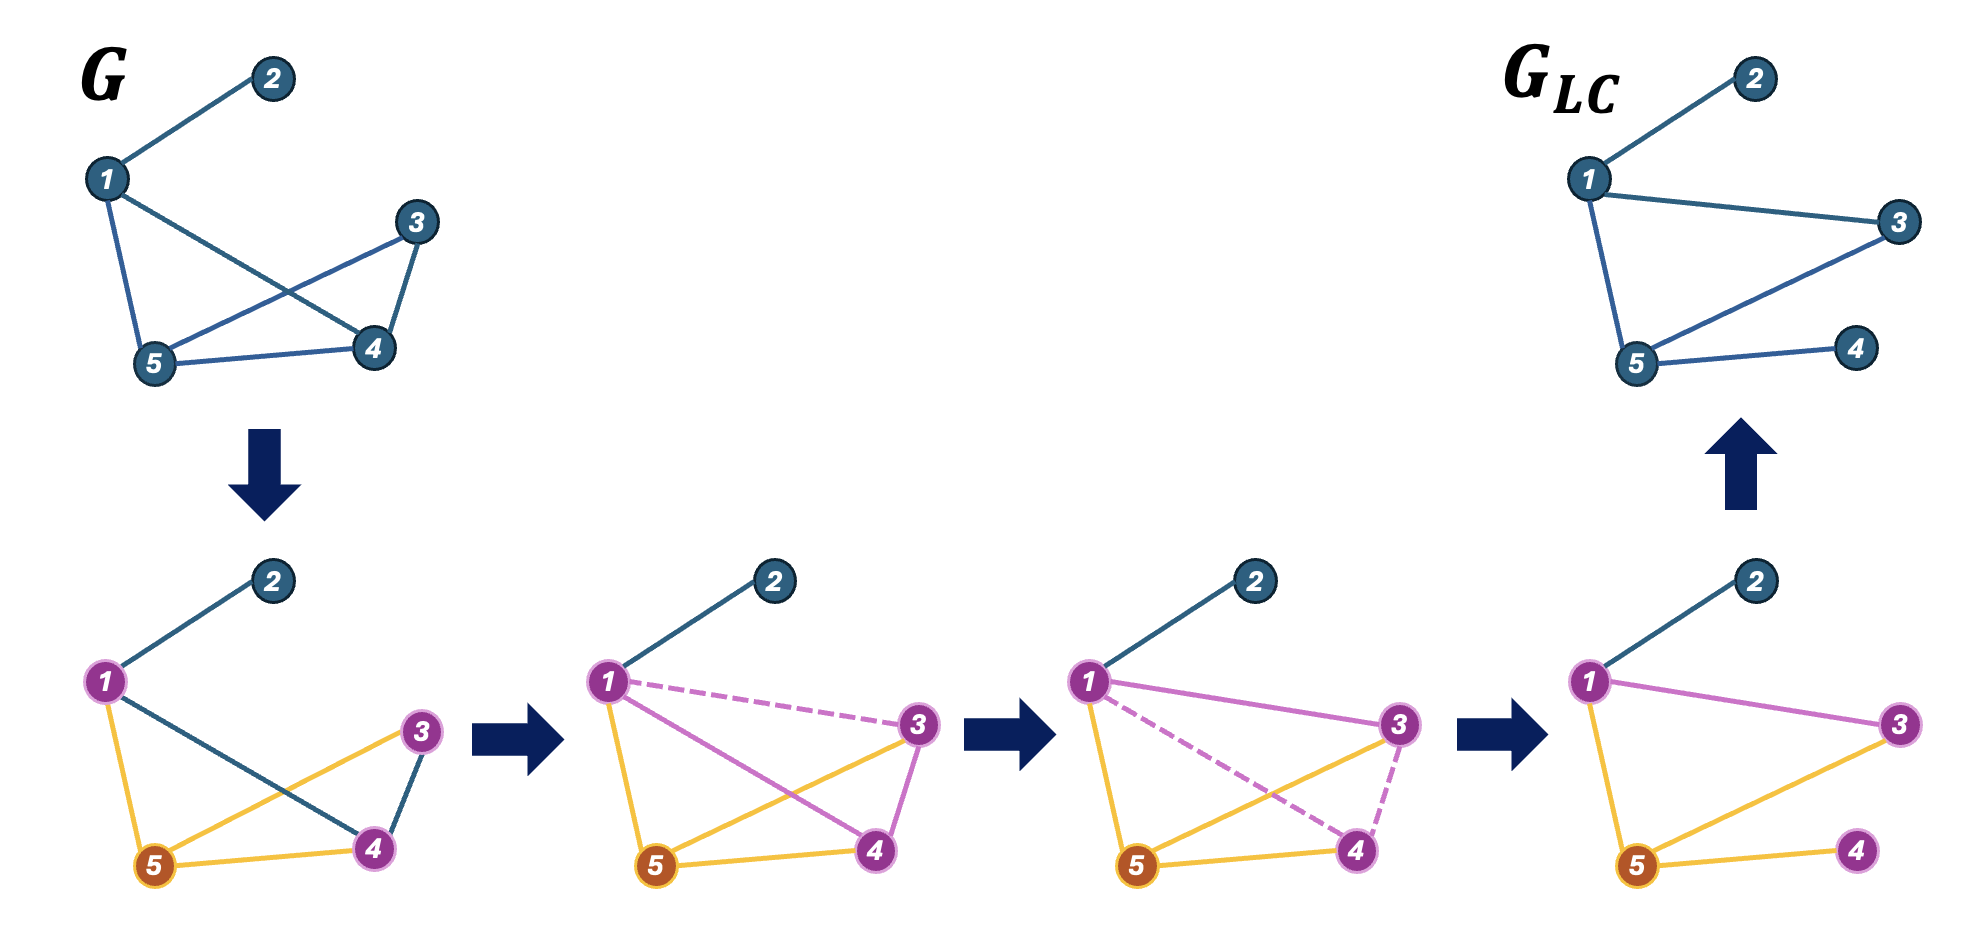
\includegraphics[width=0.75\textwidth]{Images/local_comp_demo.png}
    \caption{A guide on how the local complement of a graph yields the output graph.}
    \label{fig:lc-demo}
\end{figure}

%%%%%%%%%%%%%%%%%%%%%%%%%%%%%%%%%%%%%%%%%%%%%%%%%%%%%%%%%%%%%%%%%%%%%%%%%%%%%%%%%%%%%%%%%%%%%%%%%%%%%%%%%%%%%%%%%%%%%%%%
\newpage 
%%%%%%%%%%%%%%%%%%%%%%%%%%%%%%%%%%%%%%%%%%%%%%%%%%%%%%%%%%%%%%%%%%%%%%%%%%%%%%%%%%%%%%%%%%%%%%%%%%%%%%%%%%%%%%%%%%%%%%%%

\subsection*{Methodology}

Our work on finding all combinations of local complements on a graph $G$ will be done using a branch-and-bound scheme. This idea was inspired by \cite{hicks2006branch} with the scheme being used to 
find the maximum stable/independent set and maximum cliques. We'll instead approach the problem by finding all possible combinations of such local complements (see Figure \ref{fig:branch-scheme}). 

\begin{figure}[h!]
    \centering
    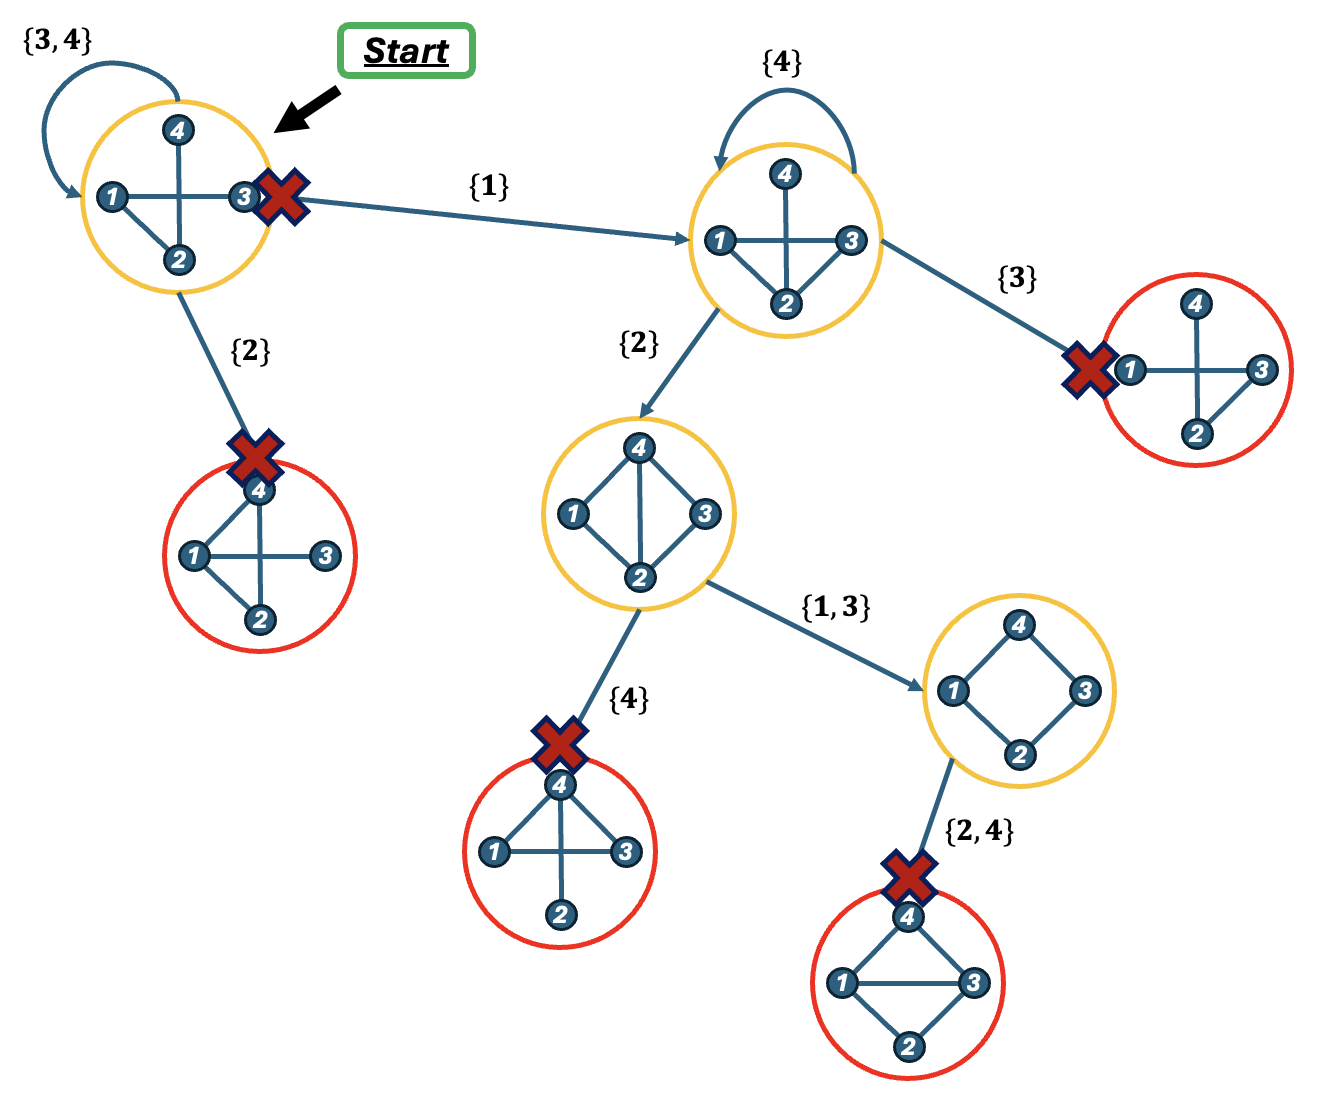
\includegraphics[width=0.6\textwidth]{Images/branch_scheme.png}
    \caption{Branch-and-bound scheme overview. Note that the graph eventually returns to the initial graph state, though it may be isomorphic to a previously seen graph.}
    \label{fig:branch-scheme}
\end{figure}

In constructing our algorithm, we define the function \texttt{isomorphic\_status}($G$) where $G$ is a checked if it's isomorphic to the previous seen graphs in \texttt{graph\_list}. Given this, we define the following function \texttt{gen\_orbits(G, lvl)} where \texttt{lvl} is the recursion level index.

\begin{algorithm}
\caption{\texttt{gen\_orbits($G$, \texttt{lvl})}}\label{alg:nic-bb}
\begin{algorithmic}
\Require{Graph $G = (V, E)$, Recursion level index \texttt{lvl}}
\Ensure{Set of all non-isomorphic graphs reachable via local complements}
\If{\texttt{is\_isomorphic($G$)}} 
    \State \texttt{return}
\EndIf
\State \texttt{graph\_list.append($G$)}
\For {$\mathbf{v} \in V(G)$}
    \If{$\left|N_{G}(\mathbf{v})\right| \leq 1$} 
        \State \texttt{continue}
    \EndIf
    \State $G_{\texttt{new}} = \texttt{gen\_local\_complement}(G, N_{G}(\mathbf{v}))$
    \State \texttt{gen\_orbits($G_{\texttt{new}}$, $\texttt{lvl}+1$)}
\EndFor
\end{algorithmic}
\end{algorithm}

\newpage 

Once all the local complements of the original graph $G$ are collected, we continue to 
collect the following information on each graph: 

\begin{enumerate}[label=(\roman*), font=\itshape]
    \item \textbf{Maximum Independent/Stable Set}
    \item \textbf{Maximum Clique}
    \item \textbf{Matchings}
    \item \textbf{Perfect Matchings}
\end{enumerate}

For these results, we use relaxed versions of their integer program formulations from \cite{conforti2014integer}. Supposing the graph $G = (V, E)$ is given, 
we have the following linear programs: 

\vspace{1em}

\begin{table}[h]
\centering
\begin{tabular}{|c|c|}
\hline
\textbf{Maximum Independent/Stable Set} & \textbf{Maximum Clique} \\
\hline
\begin{minipage}{0.45\textwidth}
\[
    \begin{aligned}
        \max \quad & \sum_{\mathbf{v} \in V} x_\mathbf{v} \\
        \text{s.t.} \quad & x_\mathbf{u} + x_\mathbf{v} \le 1 && \forall\, \mathbf{u}\mathbf{v} \in E \\
        & x_{\mathbf{v}} \geq 0 && \forall\, \mathbf{v} \in V
    \end{aligned}
\]
\end{minipage}
&
\begin{minipage}{0.45\textwidth}
\[
    \begin{aligned}
        \max \quad & \sum_{\mathbf{v} \in V} x_\mathbf{v} \\
        \text{s.t.} \quad & x_\mathbf{u} + x_\mathbf{v} \le 1 && \forall\, \mathbf{u}\mathbf{v} \notin E \\
        & x_{\mathbf{v}} \geq 0 && \forall\, \mathbf{v} \in V
    \end{aligned}
\]
\end{minipage} \\
\hline
\textbf{Matchings} & \textbf{Perfect Matchings} \\
\hline
\begin{minipage}{0.45\textwidth}
\[
    \begin{aligned}
        \max \quad & \sum_{\mathbf{e} \in E} x_\mathbf{e} \\
        \text{s.t.} \quad & \sum_{\mathbf{e} \in \delta(\mathbf{v})} x_\mathbf{e} \le 1 && \forall\, \mathbf{v} \in V \\
        & x_{\mathbf{e}} \geq 0 && \forall\, \mathbf{e} \in E
    \end{aligned}
\]
\end{minipage}
&
\begin{minipage}{0.45\textwidth}
\[
    \begin{aligned}
        \max \quad & \sum_{\mathbf{e} \in E} x_\mathbf{e} \\
        \text{s.t.} \quad & \sum_{\mathbf{e} \in \delta(\mathbf{v})} x_\mathbf{e} = 1 && \forall\, \mathbf{v} \in V \\
        & x_{\mathbf{e}} \geq 0 && \forall\, \mathbf{e} \in E
    \end{aligned}
\]
\end{minipage} \\
\hline
\end{tabular}
\end{table}

Note that in both the linear programs for both matchings and perfect matchings, we let $\delta(\mathbf{v})$ denote the set of all edges $\mathbf{e} \in E$ that have $\mathbf{v}$ is an endpoint. 

\subsection*{Computational Results}

We define each graph in our work with networkx's function \texttt{erdos\_renyi\_graph($n$, $p$)} where 
\begin{enumerate}[label=(\roman*), font=\itshape]
    \item $n$: Number of nodes defined in the graph. 
    \item $p$: Probability an edge will exist in the graph.
\end{enumerate}
Hence, $\mathbf{e} \sim \emph{Bernoulli}(p)$ for every $\mathbf{e} \in E$. 

\vspace{1em}

We start by considering how the edge density impacts the number of local complements. Each graph will have $n=8$, with edge probabilities
\[
p\in\{0.25,\,0.40,\,0.55,\,0.70,\,0.85\}.
\]

We share both the graph generated and it's corresponding results on the appearance count and the recursion over time. 

%%%%%%%%%%%%%%%%%%%%%%%%%%%%%%%%%%%%%%%%%%%%%%%%%%%%%%%%%%%%%%%%%%%%%%%%%%%%%%%%%%%%%%%%%%%%%%%%%%%%%%%%%%%%%%%%%%%%%%%%
\newpage 
%%%%%%%%%%%%%%%%%%%%%%%%%%%%%%%%%%%%%%%%%%%%%%%%%%%%%%%%%%%%%%%%%%%%%%%%%%%%%%%%%%%%%%%%%%%%%%%%%%%%%%%%%%%%%%%%%%%%%%%%

\begin{table}[h!]
\centering
\begin{tabular}{|c|c|}
\hline
\textbf{Graph} & \textbf{Plot} \\
\hline
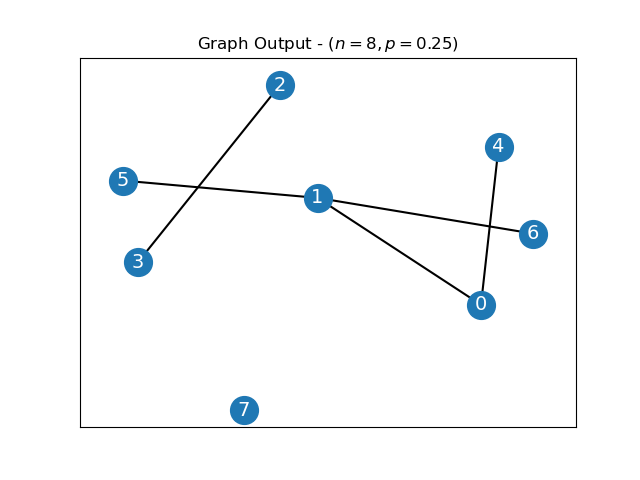
\includegraphics[width=0.75\textwidth,height=0.12\textheight,keepaspectratio]{Images/graph-p25.png} &
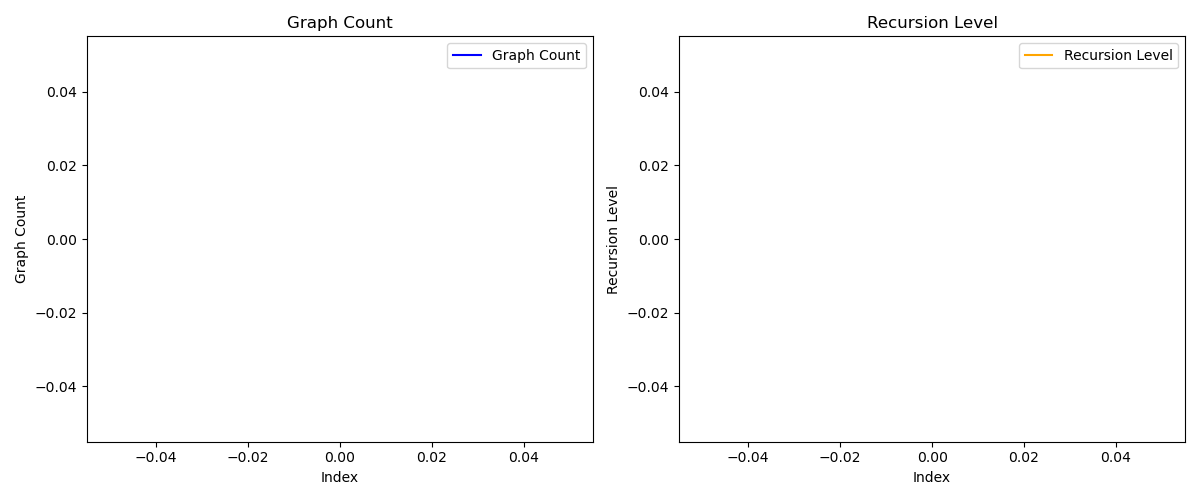
\includegraphics[width=0.75\textwidth,height=0.12\textheight,keepaspectratio]{Images/plot-p25.png} \\
\hline
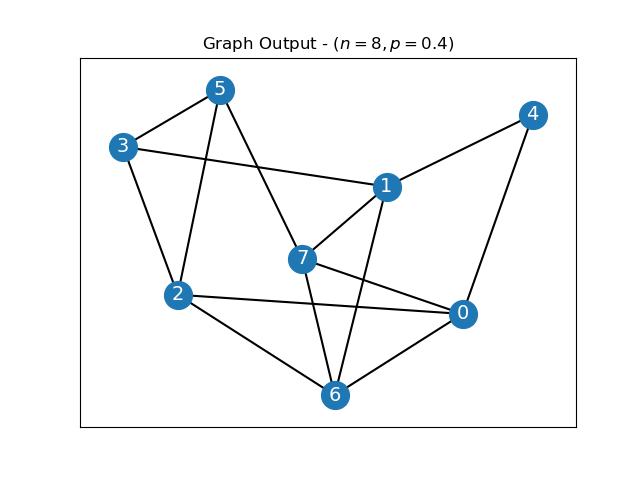
\includegraphics[width=0.75\textwidth,height=0.12\textheight,keepaspectratio]{Images/graph-p40.png} &
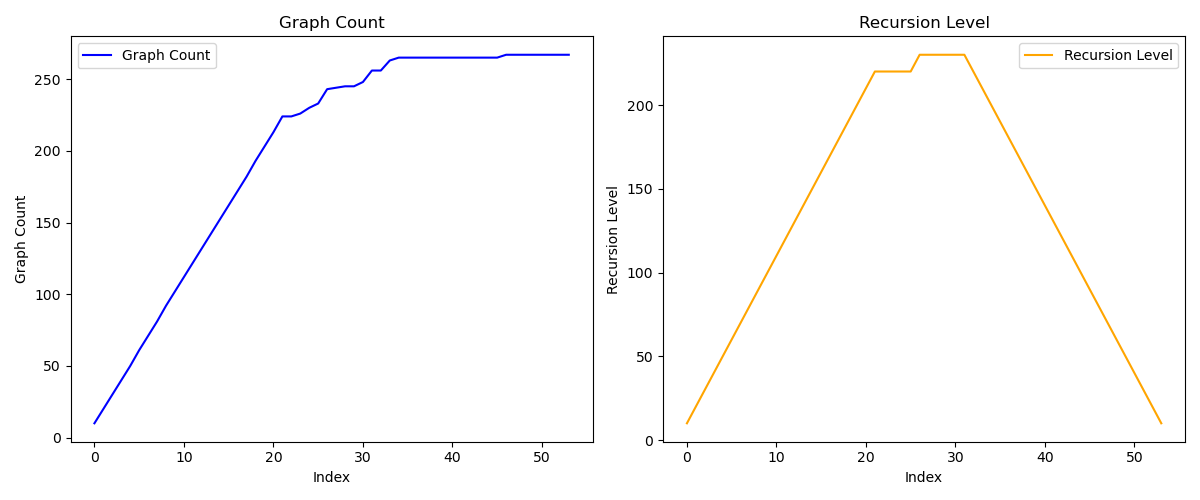
\includegraphics[width=0.75\textwidth,height=0.12\textheight,keepaspectratio]{Images/plot-p40.png} \\
\hline
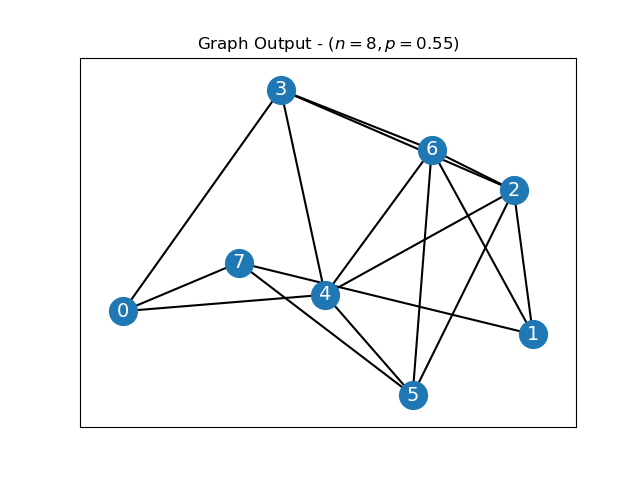
\includegraphics[width=0.75\textwidth,height=0.12\textheight,keepaspectratio]{Images/graph-p55.png} &
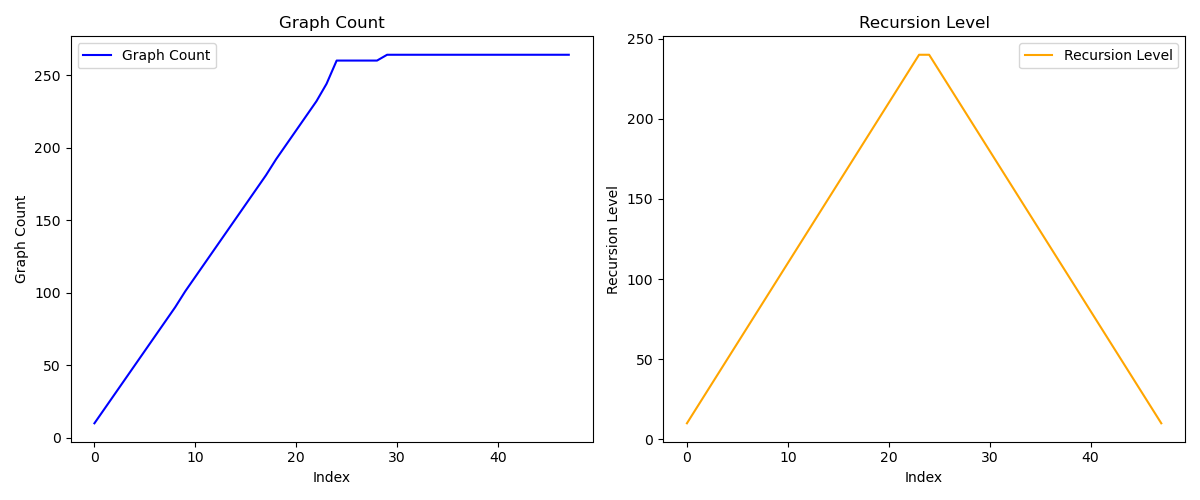
\includegraphics[width=0.75\textwidth,height=0.12\textheight,keepaspectratio]{Images/plot-p55.png} \\
\hline
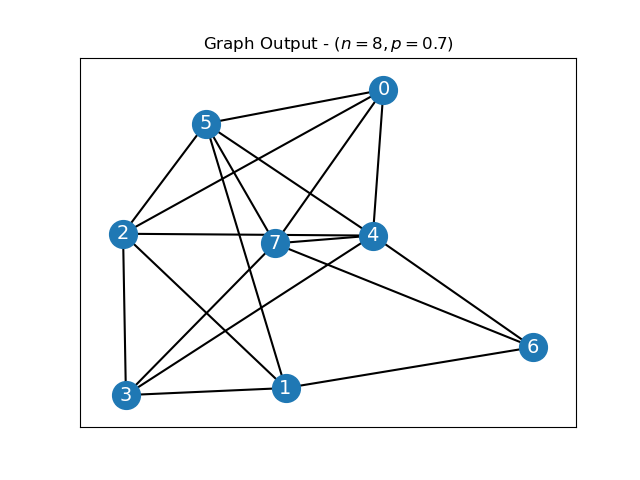
\includegraphics[width=0.75\textwidth,height=0.12\textheight,keepaspectratio]{Images/graph-p70.png} &
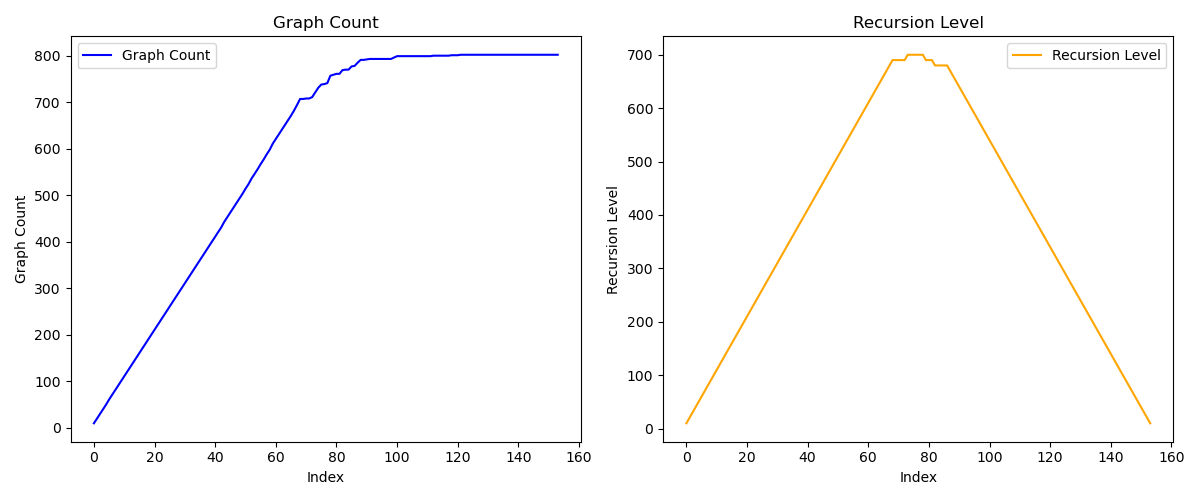
\includegraphics[width=0.75\textwidth,height=0.12\textheight,keepaspectratio]{Images/plot-p70.png} \\
\hline
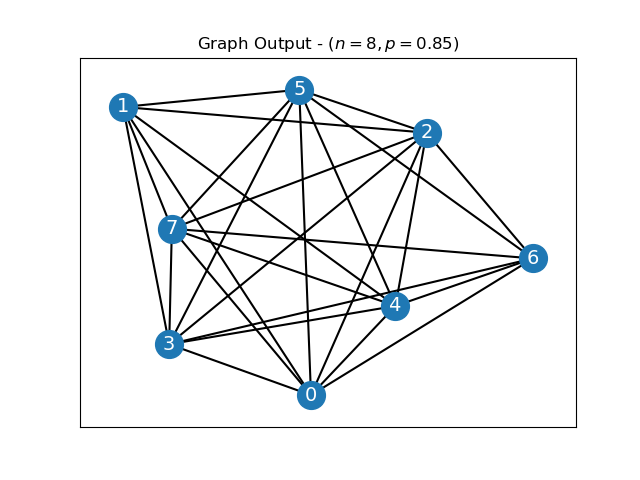
\includegraphics[width=0.75\textwidth,height=0.12\textheight,keepaspectratio]{Images/graph-p85.png} &
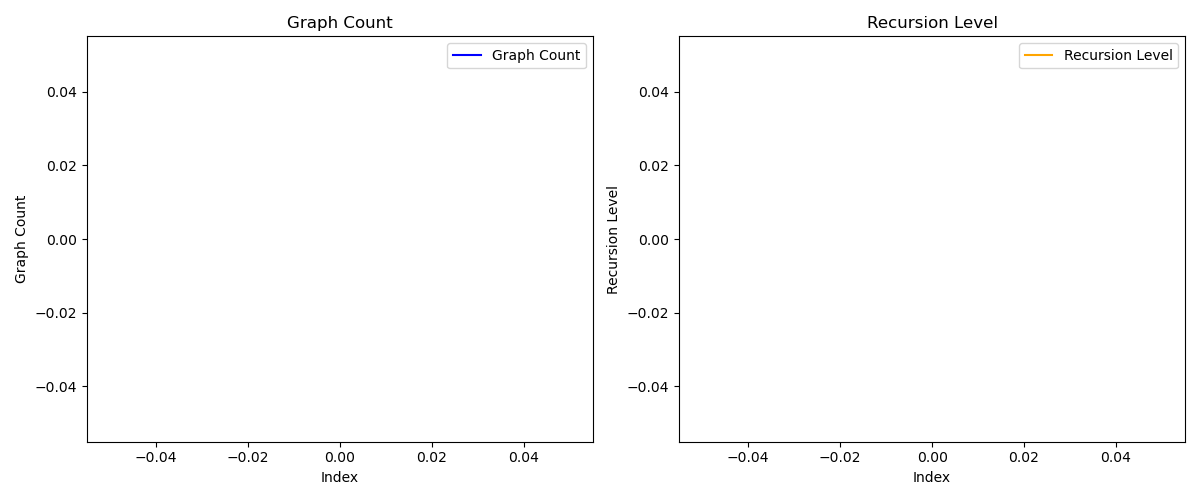
\includegraphics[width=0.75\textwidth,height=0.12\textheight,keepaspectratio]{Images/plot-p85.png} \\
\hline
\end{tabular}
\caption{Generated graphs and corresponding appearance-count plots and recursion execution for varying probabilities $p \sim \{0.25, 0.4, 0.55, 0.7, 0.85\}$. For probabilites $p = 0.25$ and $p = 0.85$, the blank plots come from the number of graphs being less than 10 as a result.}
\label{tab:graphs_plots}
\end{table}

\begin{table}[h!]
\centering
\begin{tabular}{|c|c|c|}
\hline
Probability $p$ & Time taken (s) & Final graph count \\
\hline
0.25 & 0.01 & 6 \\
0.40 & 2.24 & 267 \\
0.55 & 1.87 & 264 \\
0.70 & 17.74 & 802 \\
0.85 & 0.01 & 6 \\
\hline
\end{tabular}
\caption{Execution times and resulting head counts for each edge probability $p$.}
\label{tab:timings_counts}
\end{table}

We also studied how the matchings, cliques, and stable sets by considering $n = 8$ and $p = 0.65$. 

%%%%%%%%%%%%%%%%%%%%%%%%%%%%%%%%%%%%%%%%%%%%%%%%%%%%%%%%%%%%%%%%%%%%%%%%%%%%%%%%%%%%%%%%%%%%%%%%%%%%%%%%%%%%%%%%%%%%%%%%
\newpage 
%%%%%%%%%%%%%%%%%%%%%%%%%%%%%%%%%%%%%%%%%%%%%%%%%%%%%%%%%%%%%%%%%%%%%%%%%%%%%%%%%%%%%%%%%%%%%%%%%%%%%%%%%%%%%%%%%%%%%%%%

\begin{table}[h!]
\centering
\begin{tabular}{|c|}
\hline
\textbf{Plot} \\
\hline
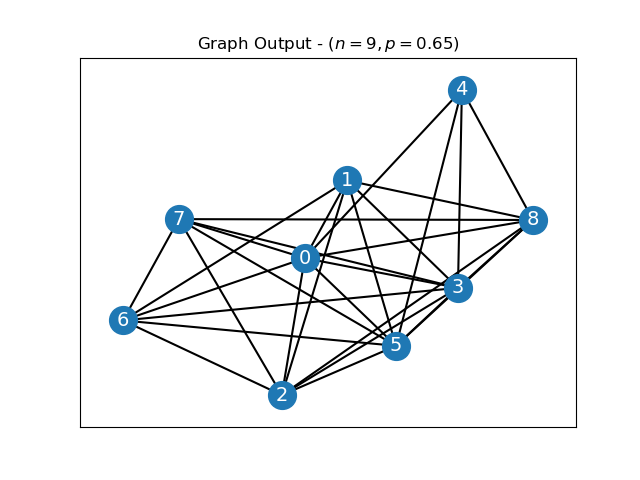
\includegraphics[width=0.4\textwidth,height=0.18\textheight,keepaspectratio]{Images/data_graph_plot.png} \\
\hline
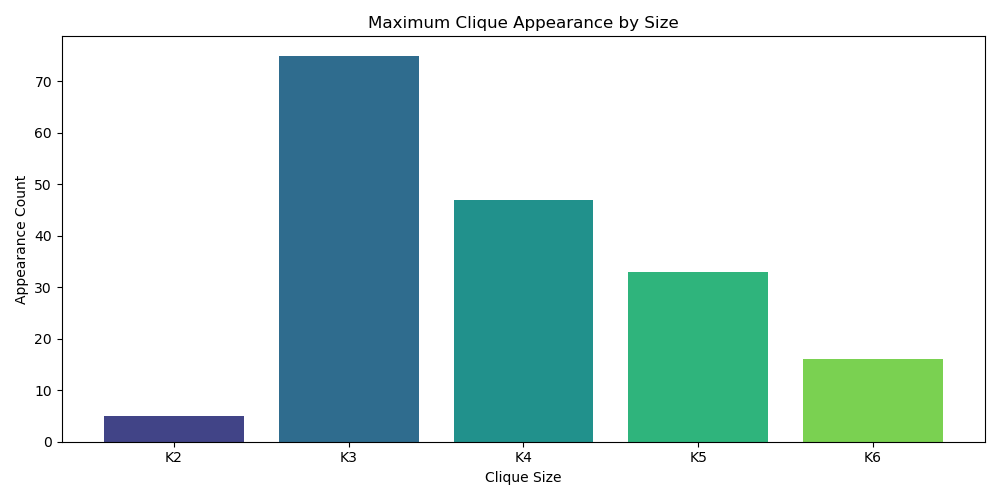
\includegraphics[width=0.4\textwidth,height=0.18\textheight,keepaspectratio]{Images/data_clique_plot.png} \\
\hline
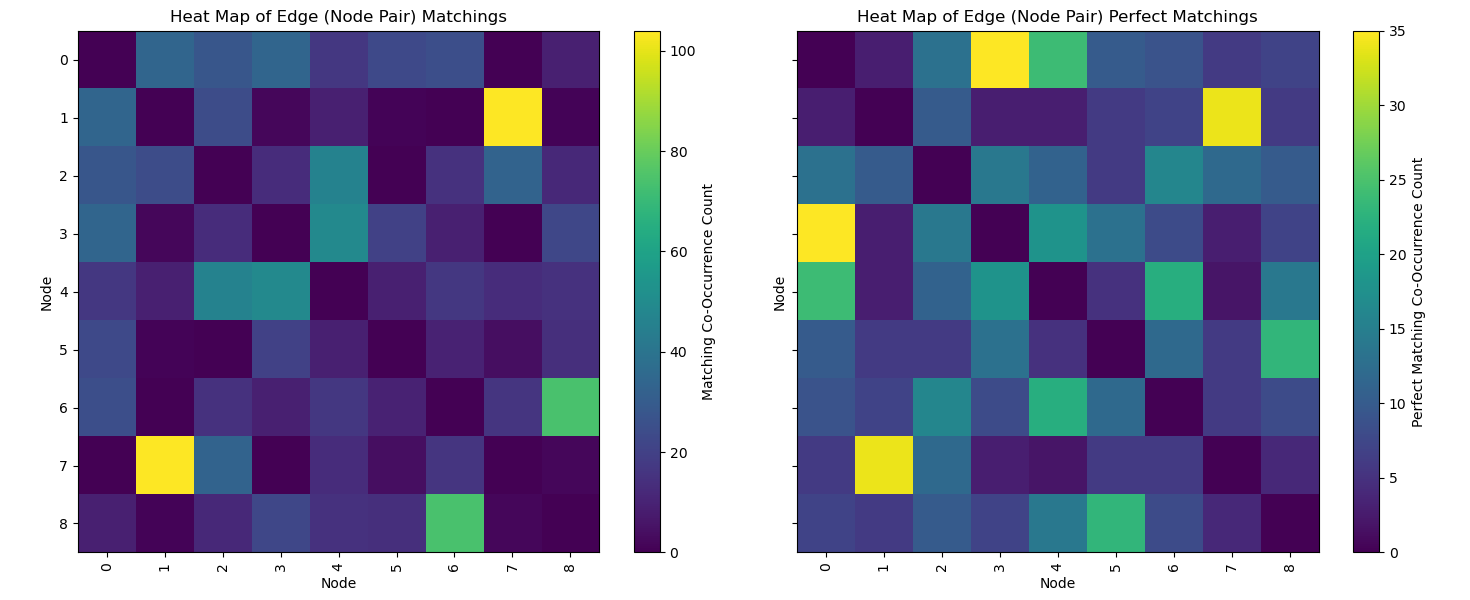
\includegraphics[width=0.4\textwidth,height=0.18\textheight,keepaspectratio]{Images/data_match_plot.png} \\
\hline
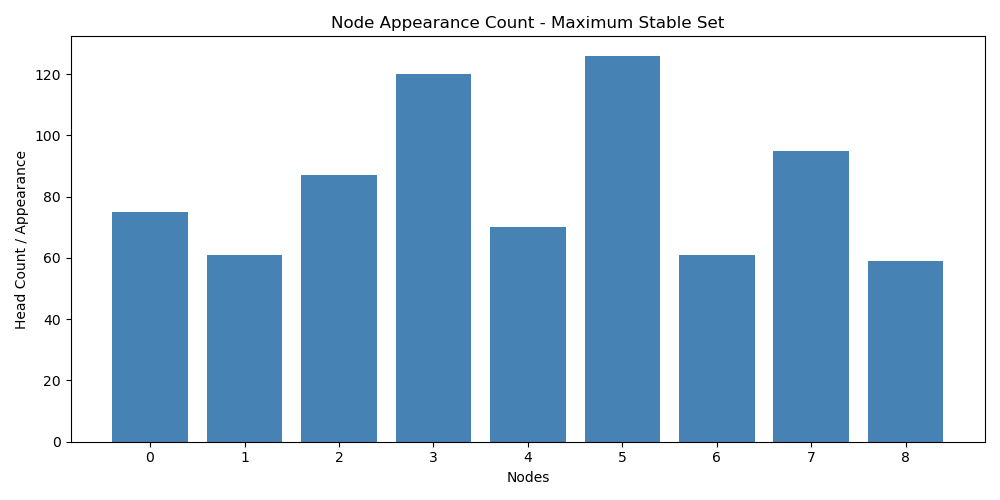
\includegraphics[width=0.4\textwidth,height=0.18\textheight,keepaspectratio]{Images/data_mis_plot.png} \\
\hline
\end{tabular}
\caption{Sample plots for a graph $G$ with nodes $n = 8$ and probability $p = 0.65$, showing the sample graph along with its plots for maximum cliques, matchings and perfect matchings, and maximum independent/stable set.}
\label{tab:data_plots}
\end{table}

\subsection*{Conclusions}

We successfully implemented and analyzed algorithms for solving fundamental graph theory problems: Maximum Clique, Maximum Matching, Perfect Matching, and Maximum Independent Set. 

\vspace{1em}

We were capable of performing the following tasks: 
\begin{enumerate}[label=(\roman*), font=\itshape]
    \item Implement all algorithms in python and tested on random graphs of varying densities.
    \item Computational complexity increases significantly with graph size, especially for NP-hard problems (Clique, Independent Set).
    \item Graph density (parameter $p$) directly impacts the size and number of solutions found.
    \item The visualization tools effectively demonstrate the structure of graphs and their corresponding solutions.
\end{enumerate}

The empirical results align with theoretical expectations, confirming the practical applicability and correctness of the implemented approaches. 

\subsection*{Limitations, Discussions, and Future Work}

Our work was limited to pure graph theory with almost no connection to quantum computing. Additionally, not much content was provided on topics seen in linear and integer programming. Given this our future will consists of the following: 

\begin{enumerate}[label=(\roman*), font=\itshape]
    \item Applying blossom inequalities to study how this affects the optimal value and its connections to qubits. 
    \item Performing a breadth-first traversal to find all non-isomorphic local complemented graphs. 
\end{enumerate}

%%%%%%%%%%%%%%%%%%%%%%%%%%%%%%%%%%%%%%%%%%%%%%%%%%%%%%%%%%%%
\newpage
%%%%%%%%%%%%%%%%%%%%%%%%%%%%%%%%%%%%%%%%%%%%%%%%%%%%%%%%%%%%

\bibliographystyle{plain}
\bibliography{references}

\end{document}